\chapter{总结与展望}
\label{cha:summarize}
\section{总结}

本论文通过针对基于Spring MVC框架开发的WEB应用系统进行应用、数据库、服务器三个层级的优化研究,如图~\ref{fig:summery}所示。
\begin{figure}[H] % use float package if you want it here
  \centering
  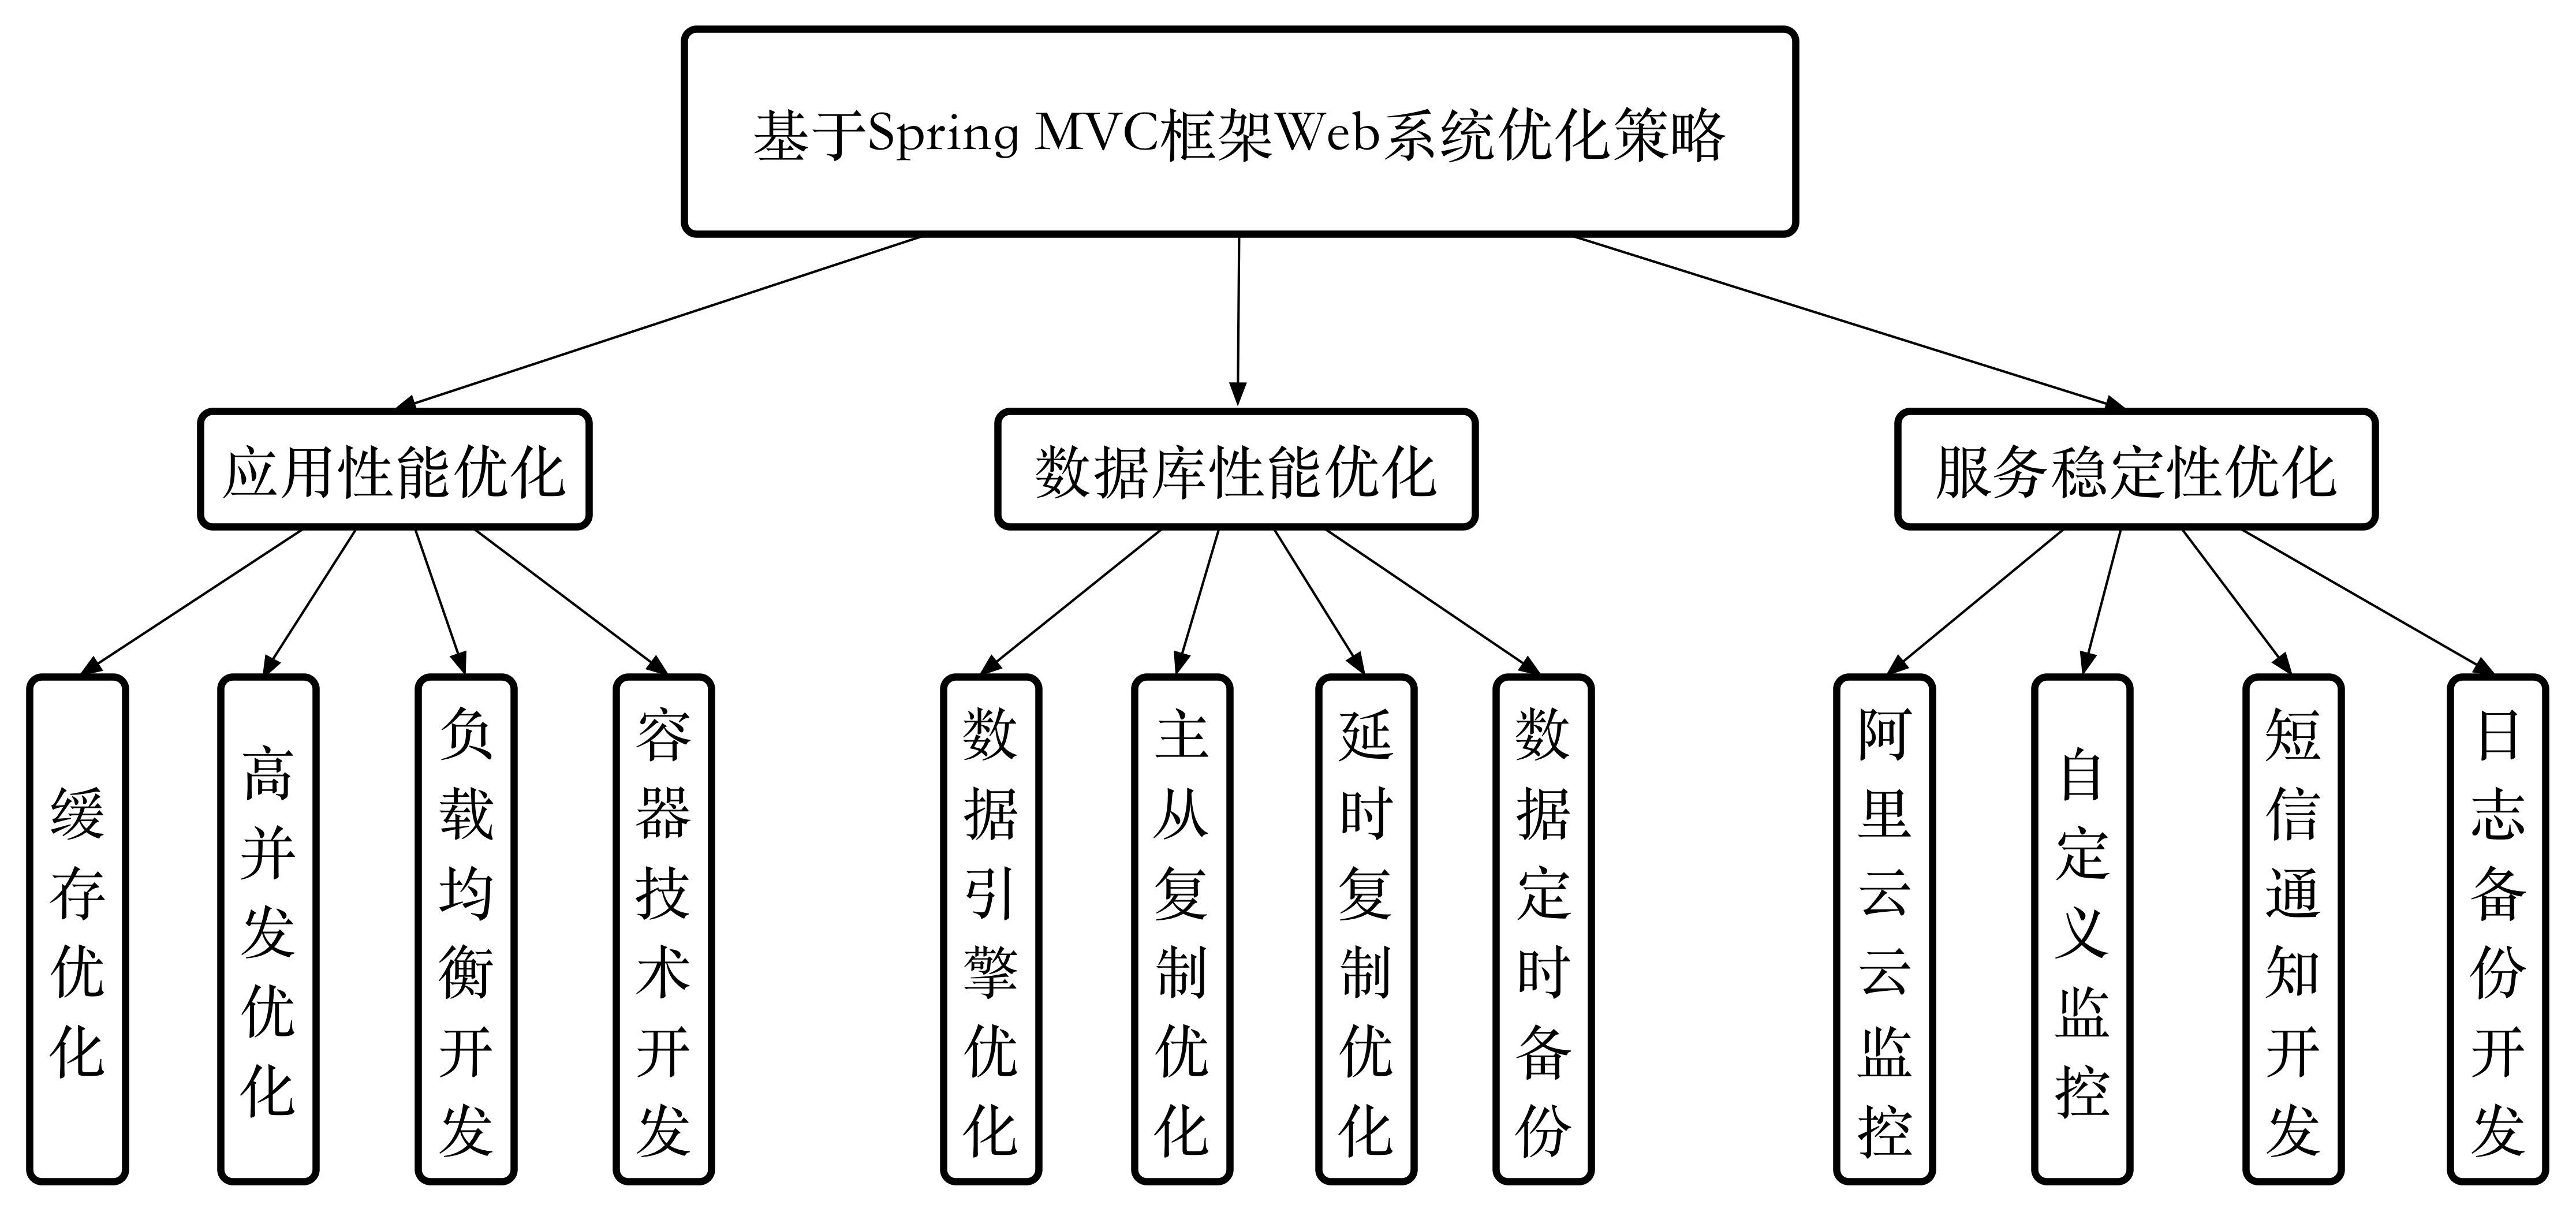
\includegraphics[width=6in]{chap06/summery}
  \caption{系统优化研究总结}
  \label{fig:summery}
\end{figure}

对于应用层面,论文通过开发Couchbase技术,将应用的基础数据缓存到Couchbase缓存中,提高了数据的加载效率并且降低了数据的压力;通过对Tomcat进行基于高并发的apr模块优化,大大提升了Tomcat对于用户请求的处理,提升了用户的访问速度;通过开发负载均衡技术,将用户的请求转发到两台应用服务器中,降低了服务器的压力,同时增强了应用的高可用性;通过开发Docker容器技术,将数据库应用、Couchbase应用以容器的方式提供服务,在新增加服务器节点的过程中提高了快速部署应用的效率,同时实现了多个服务器同一服务的集中管理,大大提高了运维人员的工作效率。

对于数据库层面,首先对数据库使用的数据引擎InnoDB引擎进行优化,在内存读取、日志、IO和其它方面提升了数据库的运行效率以及数据的稳定性;通过开发双主数据库的主从复制,提升了数据库的高可用性以及数据的完整性;通过开发延迟复制,可以最大程度的将数据进行备份,加上机遇二进制日志的恢复方式,能够在短时间内完成数据的恢复,这对于提高数据的完整行和应用的用户体验尤为重要;通过开发数据定时备份脚本,将每日的数据进行备份,以防数据丢失带来的数据损伤和经济损失。

对于服务器层面,论文通过阿里云的云监控服务,对系统的云服务器、负载均衡、网络站点以及CDN进行监控,当监控项出现异常时通知运维人员作出相应的处理,这提高了发现问题和解决服务器故障的效率,通过降低了过多流量丢失导致的经济损失;通过开发自定义监控实现对Tomcat服务的健康状态进行监测和重启,对MySQL的健康状态进行监测和根据监控情况调整数据库负载均衡损害数据库服务器的权重,并且短信通知运维人员,对于MySQL的主从同步状态进行同步状态监测并且通知运维人员;通过开发短信通知模块,实现重要信息的短信通知;通过日志备份模块的开发对Tomcat的运行日志进行定时备份并且上传到阿里云归档存储,提升运维人员在发生故障时的故障原因定位。

通过三个层面的优化策略研究,目前应用服务较优化前相比,单个服务器的负载达到了比较好的程度,应用的访问速度提升了接近20\%,新版的部署时间节省了50\%。

具体的数据对比在后期的论文完善过程中进行补充。

\section{展望}

虽然通过本论文的优化,WEB应用的性能得到了大大的提升,但是目前的WEB应用系统依然有很大的改进空间。
\begin{enumerate}

\item 搭建基于Nginx的前端服务器,由于Nginx在高并发的处理和静态文件的处理速度方面以及安全性方面的性能均优于Tomcat对静态页面处理,因此搭建Nginx服务器处理用户的请求,将前端的页面请求直接提供给用户,后端的请求通过转发到Tomcat获取数据的处理结果。这样对于应用的访问速度还能进一步的提高,对于DDos攻击也能起到一定程度的防御\cite{reese2008nginx}。

\item 对于数据库的性能而言,除了自身的引擎提高之外,还可以通过读写分离来提高数据库的响应和降低数据库的负载\cite{刘进京2016mysql}。通过使用MaxScale插件,实现数据库请求的读写分离。具体的流程如图~\ref{fig:maxscale}所示。

\begin{figure}[H] % use float package if you want it here
  \centering
  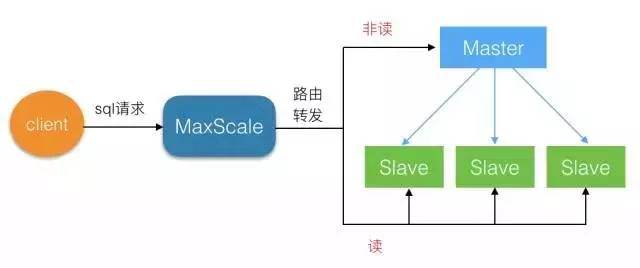
\includegraphics[width=5in]{chap06/maxscale}
  \caption{数据库读写分离流程}
  \label{fig:maxscale}
\end{figure}

MaxScale会根据用户的请求将读取的请求和非读取的请求转发到不同的数据库中,其中读取的请求转发到slave库中,其它请求转发到master库中,实现数据的读写分离。

\item 除了通过读写分离的方式提升数据库的效率以外,在数据库稳定性方面可以通过LiquiBase软件来实现数据库重构和迁移的操作,它可以在很大程度上保证当数据库之间出现数据不一致的情况时,能够自动的实现数据的同步和迁移,避免了人工干预导致的其它问题。

\item 本论文虽然用了阿里云的云监控实现了服务状态的监控,但是服务的自动failover工作却没有实现,目前还是通过人工干预来进行故障恢复。在以后的项目开发中,可以充分开发阿里云API的故障检测和自动failover系统,通过云监控的API去监控服务的状态,当出现故障时,自动调用failover程序通过故障服务的API接口进行故障的转移或者恢复,这对于提高故障的解决和WEB应用的高可用有更大的价值。

\end{enumerate}